\documentclass[border=4pt]{standalone}
\usepackage{tikz}
\usetikzlibrary{arrows.meta}
\begin{document}
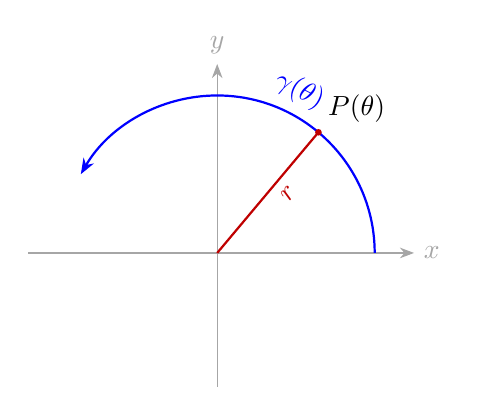
\begin{tikzpicture}[auto,axis/.style={-{Stealth[length=1.8mm]},gray!70},curve/.style={-{Stealth[length=2mm]},thick}]
  \draw[axis] (-2.4,0) -- (2.5,0) node[right] {$x$};
  \draw[axis] (0,-1.7) -- (0,2.4) node[above] {$y$};
  \draw[curve,blue] (2,0)
    arc[start angle=0,end angle=150,radius=2cm]
    node[pos=.42,sloped] {$\gamma(\theta)$};
  \draw[red!75!black,thick] (0,0) -- (50:2cm)
    node[pos=.58,sloped,swap] {$r$};
  \fill[red!75!black] (50:2cm) circle (1.2pt);
  \node[above right] at (50:2cm) {$P(\theta)$};
\end{tikzpicture}
\end{document}
